%!TEX root = ../tudkom_students__201804_v1.4.tex
\chapter{Hintergrund}
\label{ch:background}
%This chapter should give a comprehensive overview on the background necessary to understand the thesis.
% 5 pages

\section{Sensor}
% Beschleunigungssensor und Gyrosensor
Um Gelenkstellungen anzugeben, wird eine Position und Rotation gebraucht.
Diese Daten werden von einem Beschleunigungssensor und einem Gyrosensor erfasst und bestehen aus je 3 Achsen.
Die Sensoren sind platz- und energiesparend zusammen in einem Chip, der Inertialen Messeinheit (IMU), erhältlich.
Im Folgenden wird ein Einblick in die Funktionsweise der beiden Sensorentypen gegeben.

\subsection{Beschleunigungssensor}
Beschleunigungssensoren können die Beschleunigung messen, die auf den Sensor einwirkt.
Im Bereich der kleinen Bauteile werden zwei Techniken dafür eingesetzt.\\
Beim kapazitiven Sensor, der in Abbildung \ref{fig:pic_accel_kapa} illustriert ist, wird eine Masse senkrecht-federnd parallel zu einer Platte befestigt.
Mit der Platte bildet die Masse einen Kondensator.
Bei einer Beschleunigung bewegt sich die Masse zur Platte hin oder davon weg und die Kapazität des Kondensators ändert sich.
Durch diese Änderung lässt sich dann der Wert für die Beschleunigung berechnen. \cite{site_mems}
\begin{figure}[hbtp]
	\centering
	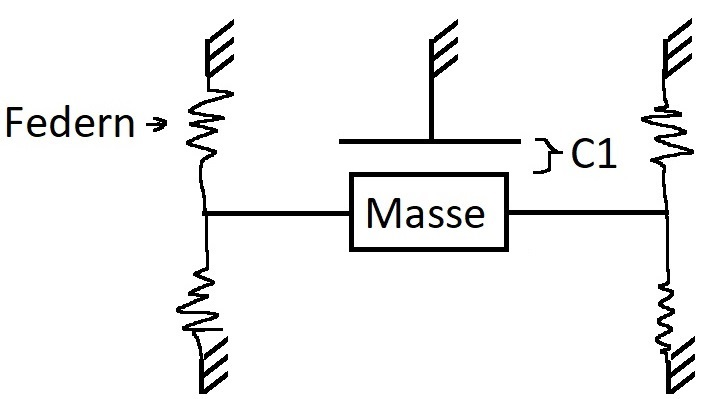
\includegraphics[width=0.33\linewidth]{res/kinAccel.jpg}
	\caption{Funktionsweise eines kapazitiven Beschleunigungssensors. Basierend auf \cite{site_sensorbild}}
	\label{fig:pic_accel_kapa}
\end{figure}\\
Beim piezoresistiven Sensor, der in Abbildung \ref{fig:pic_accel_pie} dargestellt ist, wird ein Stoff genutzt, der bei Dehnung seinen Widerstand ändert (Piezoresistiver Effekt).
Eine Masse wird an diesen piezoresistiven Stoff befestigt.
Durch die Beschleunigung wird der Stoff gedehnt, wodurch die Beschleunigung durch die Änderung des Widerstands berechnet werden kann. \cite{site_dms}
\begin{figure}[hbtp]
	\centering
	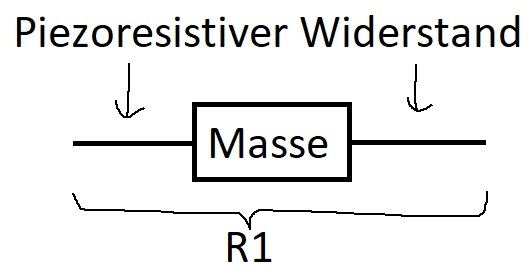
\includegraphics[width=0.25\linewidth]{res/prAccel.jpg}
	\caption{Funktionsweise eines piezoresistiven Beschleunigungssensors. Basierend auf \cite{site_sensorbild}}
	\label{fig:pic_accel_pie}
\end{figure}

\subsection{Gyrosensor}
Mit einem Gyrosensor, zu sehen in Abbildung \ref{fig:pic_gyro}, wird die Drehung gemessen.
Eine Masse wird dabei senkrecht-federnd parallel zu einer Platte befestigt, sodass wieder ein Kondensator entsteht.
Parallel zu der Platte wird die Masse von außen zum Schwingen gebracht.
Dieses Konstrukt gibt es ein zweites Mal in die andere Richtung schwingend.
Durch die Subtraktion der beiden Kapazitäten der Kondensatoren kann die Drehgeschwindigkeit berechnet werden.
Da die Schwingung gegensätzlich ist, bewegen sich die Massen bei einer Drehung in entgegengesetzte Richtungen (Coriolis Effekt) und die Differenz der Kapazitäten ändert sich.
Bei einer geraden Beschleunigung bewegen sich beide Massen in die selbe Richtung und die Differenz der Kapazitäten ändert sich nicht. \cite{gyrosensor}
\begin{figure}[hbtp]
	\centering
	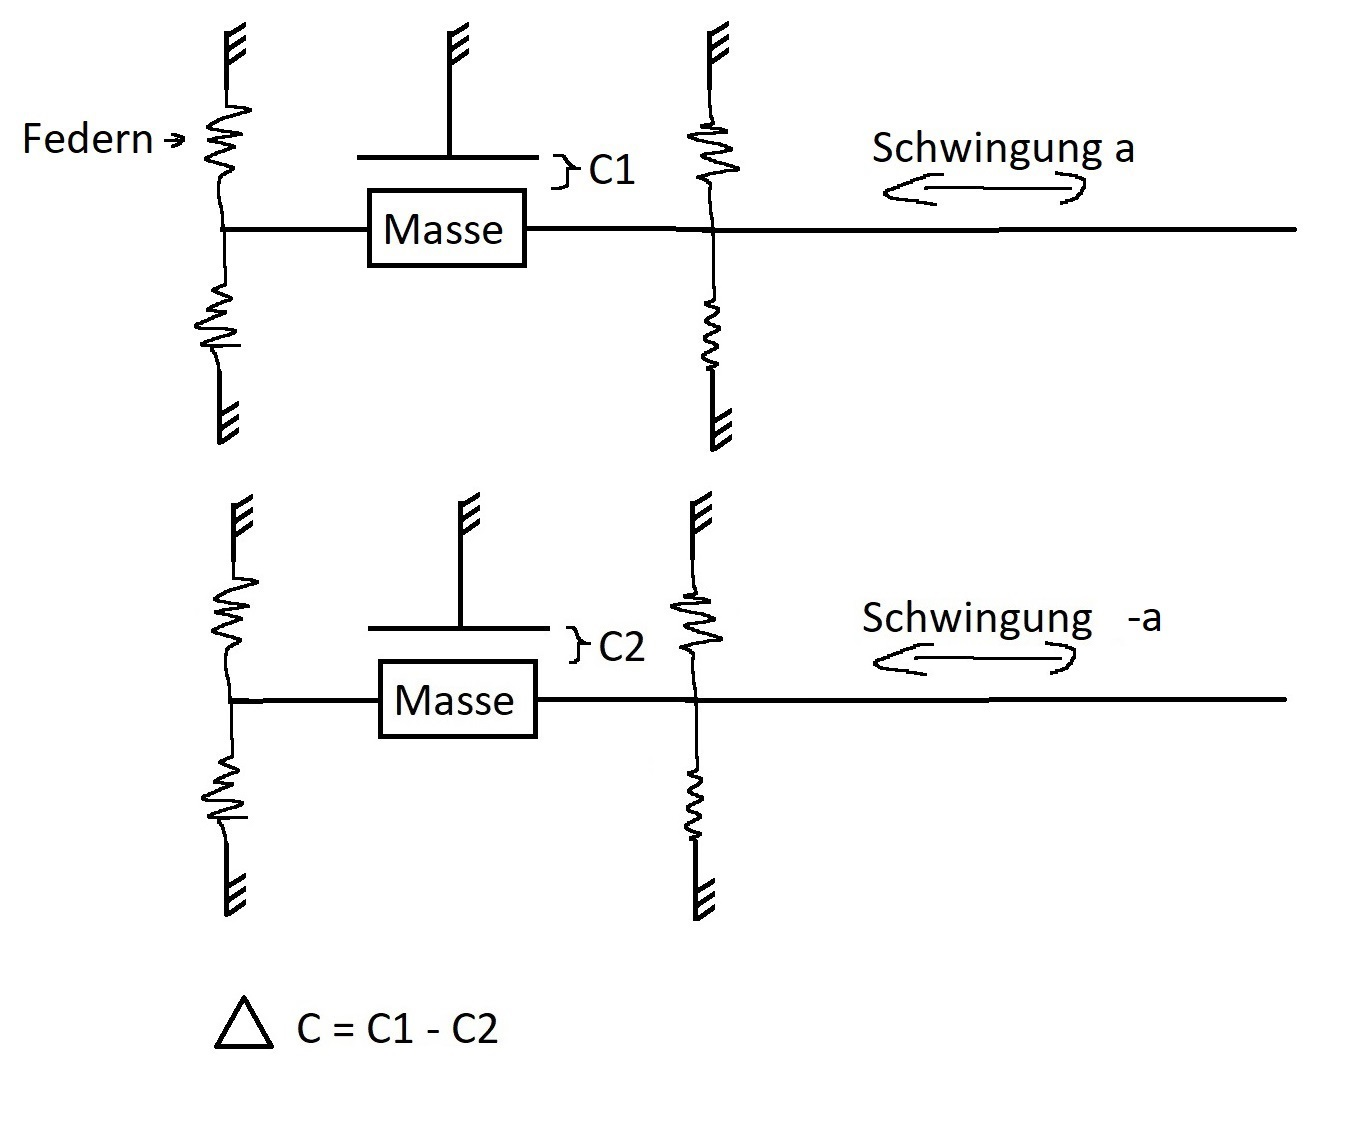
\includegraphics[width=0.65\linewidth]{res/gyro.jpg}
	\caption{Funktionsweise eines Gyrosensors [eigene Darstellung]}
	\label{fig:pic_gyro}
\end{figure}\\
Da konstant eine Schwingung auf der Masse gehalten werden muss, damit der Coriolis Effekt auftritt, benötigt der Gyrosensor mehr Strom als der Beschleunigungssensor.

\section{Chipkommunikation}
% I2C und SPI
Eine IMU enthält in der Regel keine programmierbare Chiparchitektur sondern wird mit einer Mikrocontroller Unit (MCU) betrieben.
Die MCU beinhaltet unter anderem eine Recheneinheit und einen Programmspeicher.
Zur Kommunikation zwischen IMU und MCU kann wiederum zwischen einigen Systemen gewählt werden.
Die verwendeten IMUs unterstützen die weit verbreiteten Master-Slave-Systeme Inter-Integrated Circuit (I2C) und Serial Peripheral Interface (SPI), die beide auf der gewählten MCU laufen.
Die Chipkommunikation läuft in der Regel mit einer langsameren Frequenz als die Recheneinheit.
Einerseits kann die Übertragungsfrequenz von der Software emuliert werden, indem Takte der Recheneinheit übersprungen werden, wodurch die Recheneinheit nicht in den Schlafmodus gehen kann.
Andererseits kann die Recheneinheit einen weiteren Chip nutzen, der mit einem Buffer die Übertragung effizient abarbeiten kann.

\subsection{I2C}
Bei dem I2C-Protokoll sieht die Verdrahtung Serial Clock (SCL) und Serial Data (SDA) mit Pull-Up Widerständen vor.
Der Master startet eine Datenübertragung mit START indem er SDA auf Masse zieht während SCL auf Spannung ist.
Dann gibt der Master den Takt auf SCL vor.
Es folgt ein Paket mit 7 Bits für die Slaveadresse und 1 Bit für Read oder Write.
Der Slave bestätigt den Empfang mit ACK, indem er SDA für eine Bitübertragung auf Masse zieht.
Nun können 8-Bit-Datenpakete übertragen werden, die jeweils mit ACKs bestätigt werden.
Zum Schluss sendet der Master STOP, indem er SDA auf Spannung setzt während SCL auch auf Spannung ist. \cite{manual_i2c}

\subsection{SPI}
Bei dem SPI-Bussystem sind Chip Select (CS), Serial Clock (SCK), Master-In-Slave-Out (MISO) und Master-Out-Slave-In (MOSI), meist mit Pull-Up Widerständen, verkabelt.
Der Master startet die Übertragung, indem er CS auf Masse zieht und anschließend auf SCK den Takt vorgibt.
Auf MISO kann der Slave dann Daten zum Master schicken und auf MOSI der Master Daten zum Slave.
Um die Übertragung zu beenden, wird CS vom Master wieder auf Spannung gezogen. \cite{site_micSpi}

\section{Endgerätekommunikation}
% BLE und Mesh
Damit die Daten von der MCU zum Endgerät kommen, wird ein weiteres Protokoll benötigt.
Es wurde Bluetooth Low Energy (BLE) gewählt.
Weiterhin wurde ermöglicht, dass zukünftig auf Bluetooth Mesh (BT Mesh) gewechselt werden kann.
Die Entscheidung wird im Abschnitt \ref{ch:bleAndMesh} begründet.

\subsubsection{Bluetooth Low Energy}
BLE ist eine Abwandlung von Bluetooth, die für geringen Energieverbrauch optimiert ist.
Geräte können dabei die Rolle von der Central oder Peripheral einnehmen, die einem Master-Slave Protokoll gleichkommen.
Um eine Datenverbindung zu starten, kündigt sich die Peripheral auf den drei Advertising Frequenzen an, während die Central diese Frequenzen abhört.
Die Parameter dafür, zum Beispiel die bis zu 31 Byte große Payload, werden im Generic Access Profile (GAP) eingestellt.
Die Central kann auf das Advertisen der Peripheral antworten und sich mit ihr verbinden. \cite{site_adabt}\\
Nach dem Verbindungsaufbau gibt die Central eine Geschwindigkeit vor.
Die Geschwindigkeit besteht aus einem Connection Interval, einer Slave Latency und einem Supervision Timeout.
Das Connection Interval beschreibt in welchen Zeitabständen die Datenbursts passieren.
Die Slave Latency bestimmt, wie oft die Peripheral die Datenbursts pausieren kann, um Energie zu sparen, falls keine Daten gesendet werden müssen.
Der Supervision Timeout besagt, nach welcher Zeit eine Verbindung als abgebrochen gilt, wenn eine Seite nicht mehr antwortet.
Es gelten die Gleichungen \ref{eq:supTim1} bis \ref{eq:supTim2}.
\begin{gather}
  \label{eq:supTim1}
	7.5 ms \leq Connection Interval \leq 4 s\\
	0 \leq Slave Latency \leq 499\\
	100 ms \leq Supervision Timeout \leq 32 s\\
  \label{eq:supTim2}
	Supervision Timeout > Connection Interval * (1 + Slave Latency)
\end{gather}
Später kann einerseits die Peripheral neue Geschwindigkeiten vorschlagen, die von der Central angenommen oder abgelehnt werden, oder andererseits die Central neue Geschwindigkeiten von sich aus bestimmen. \cite{site_tigap}\\
Bei einer Verbindung stellt die Peripheral Services zur Verfügung, die aus Characteristics bestehen.
Jeder Service und jede Characteristic ist im Generic Attribute Profile (GATT) definiert und hat eine eindeutige ID (UUID).
Die UUID ist 16 Bit groß, wenn sie aus den vordefinierten Profilen besteht oder 128 Bit für eigene Definitionen.
Eine Characteristic repräsentiert einen Wert und kann im Lese- und Schreibzugriff eingeschränkt werden.
Die Central kann das notificate- oder indicate-Bit setzen, wodurch die Peripheral Änderungen des Wertes mitteilt, wobei beim Indicate der Empfang der Updates von der Central bestätigt werden muss. \cite{site_norChara}\\
BLE arbeitet nach einem Schichtenmodell ähnlich dem OSI-Schichtenmodell.
Während GATT und GAP auf der oberen Schicht liegen, liegt das Logical Link Control and Adaptation Layer Protocol (L2CAP) in der Mitte.
Die Pakete der oberen Schicht werden im L2CAP in Päckchen aufgeteilt.
Ein Päckchen besteht aus Header und Data und hat die Größe der Maximum Transmission Unit (MTU-Größe).
Falls das Paket nicht komplett in Data passt, werden mehrere Päckchen erstellt.
Der Header bei einem Notify-Paket ist 3 Byte groß. \cite{site_til2cap}

\subsubsection{Bluetooth Mesh}
BT Mesh erweitert BLE insoweit, als dass die Datenpakete über ein Mesh-Netwerk geflutet werden.
Der Vorteil davon ist, dass die Reichweite erhöht wird, da Pakete über Zwischenknoten gesendet werden können und, dass die Stabilität steigt, da einzelne Routen ausfallen können.
Nachteilig ist, dass der Energieverbrauch der Geräte höher ist, da sie seltener in den Schlafmodus können, weil sie Daten von anderen Knoten übertragen müssen.
Über Proxy-Knoten können BLE-Geräte eingebunden werden, die BT Mesh selber nicht unterstützen. \cite{site_mesh}

\section{Lithiumknopfzelle}
Zur Spannungsversorgung wird eine Knopfzelle aus Lithium genutzt.
Die Knopfzelle gibt es in verschiedenen Größen.
Die gängigsten Größen CR2032, CR2430 und CR2450 eignen sich dafür gut.
Die mittleren beiden Ziffern geben jeweils den Durchmesser und die hinteren beiden Ziffern die Dicke in Millimeter an.
Da sich dementsprechend die Kapazität verändert, sind in der Tabelle \ref{tab:knopfzellen} die Kapazitäten von stellvertretenden Modellen gelistet.
Alle Modelle haben eine Nennspannung von 3 V und gelten unter 2 V als entladen.
Durch ihre Selbstentladung von < 1 \% pro Jahr, sind sie lange haltbar. \cite{datasheet_ds6450}
\begin{table}[hbtp]
	\captionof{table}{Typische Kapazität von Knopfzellen verschiedener Größen}
	\label{tab:knopfzellen}
	\centering
	\begin{tabular}{l|l}
		Größe & Typische Kapazität\\
		\hline
		CR2032 & 230 mAh \cite{datasheet_ds6032}\\
		CR2430 & 300 mAh \cite{datasheet_ds6430}\\
		CR2450 & 620 mAh \cite{datasheet_ds6450}\\
	\end{tabular}
\end{table}
